\documentclass[11pt]{article}
\usepackage[
  paperheight=2.125in, 
  paperwidth=5.5in,
  margin=.3in
]{geometry}
\usepackage{tikz,graphicx}




\begin{document}
\pagestyle{empty}

\paragraph{Ex \#1} 

You hike 20 meters east and then 40 meters north.  What is your displacement (magnitude and direction)?

\pagebreak

\paragraph{Ex \#2} 

You row east across a river at a speed of 7 m/s.  The river flows north at a speed of 3 m/s.  From the perspective of someone standing on the shore, what is your velocity (magnitude and direction)?

\pagebreak

\paragraph{Ex \#3} 

A ball is thrown with an initial resultant velocity of 12.5 m/s at angle 37$^\circ$ above horizontal.  Calculate the $x$- and $y$- components of the ball's initial velocity.


\pagebreak

\paragraph{Ex \#4} 

An airplane comes in for a landing at a speed of 67 m/s.  Its angle is 15 degrees below horizontal.  Calculate the $x$- and $y$- components of the airplane's velocity.

\begin{tikzpicture}
  \node at (0,0) 
    {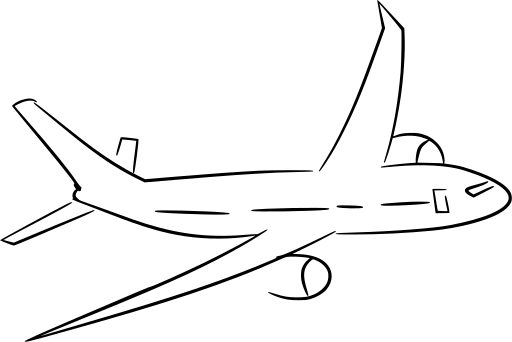
\includegraphics[angle=-15,origin=c,width=1.5cm]{airplane.png}};
  \draw[->,red,thick] (.6,-.2) coordinate (a)
    -- ++(-15:1.05) 
    node[anchor=north,rotate=-14] {\footnotesize 67 m/s} 
    -- ++(-15:1) coordinate (b);
  \draw[dashed, thin] (a) -- ++(3,0);
  \draw[brown] (-1,-1.1) -- ++(7,0);
  \node at (2.1,-.4) {\footnotesize $15^\circ$};
\end{tikzpicture}


\end{document}